\chapter{Niveau 3 : La Tombe Inférieure}\label{n3}
\section{Structure}
Il y a deux chemins principaux "horizontaux" et trois "verticaux".
Le donjon bifurque et reboucle.

Il est possible de remonter à la surface comme de plonger plus profond.
Ou même de revenir de là où l'on est parti.
Cet étage est indubitablement plus dangereux que les précédents.

La diplomatie et le troc font également leur apparition, de même que les \nameref{monster:n3:errants}.
Vous pouvez explorer les niveaux 1 et 2 à votre rythme, mais passer trop de temps au Niveau 3 revient à prendre des risques inconsidérés.

La conclusion de cet étage est ouverte : vous pouvez ajouter du contenu pour étendre ce donjon autant que vous le souhaitez.
Arrivé là, si vous êtes un nouveau MJ ou débutant en jeux OSR, vous devriez être prêt à écrire votre propre donjon.

\section{Zones Thématiques}
\subsection{Les Terriers Gobelins}
Les Gobelins Fongiques sont le miroir des PJ, leur opposé.
Ils se complaisent dans la crasse, revivent sans cesse et commettent toujours les mêmes erreurs.
Ils sont affamés, stupides, superstitieux et meurtriers, mais néanmoins attachants.
Les terriers sont l'irruption d'un barbarisme bruyant et enthousiaste dans la civilisation froide et moribonde.



Décrivez les terriers tant par le bruit que par l'odeur.
Ça pue.
Vous allez puer si vous vous attardez ici, et la Tombe des Rois Serpents n'est pas pourvue de bains.
Des petits yeux de gobelins dans la pénombre.
Des dents cliquetantes et des couteaux aiguisés.

\ifmulticolEnd
\begin{center}
  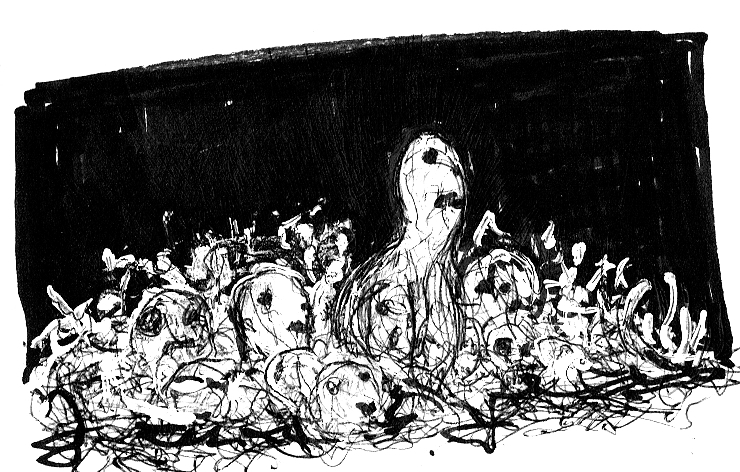
\includegraphics[width=0.5\columnwidth]{pics/goblin_pit.jpg}
\end{center}
\ifmulticolStart

\vfill
\pagebreak

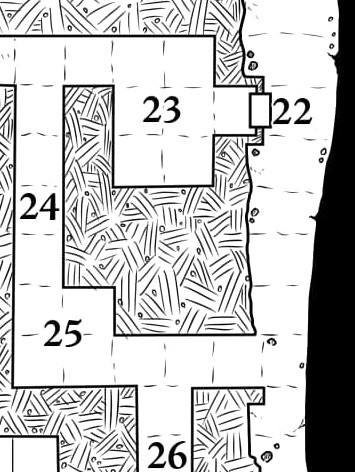
\includegraphics[width=\columnwidth]{pics/map_22-25.jpg}
\subsection{22 : Porte de Pierre}\label{n3:s22}
\begin{itemize}
  \item Enfoncée d'1,50m dans le mur
  \item Maintenue fermée par une lourde barre de pierre côté gouffre.
  \item En arrivant par l'autre côté, la porte ne peut être ouverte sans être détruite.
  \item \textbf{Piège :}
  \begin{itemize}
    \item Même que \nameref{n1:s5}
    \item Marteau vers l'extérieur :
    \begin{itemize}
      \item 1D6 dommage \textbf{puis :} (sauvegarde contre la mort +2 annule)
      \item Poussé dans le gouffre (sauvegarde contre la mort annule)
    \end{itemize}
  \end{itemize}
\end{itemize}

\subsection{24 : Couloir}\label{n3:s24}
\begin{itemize}
  \item Couloir de 3m sur 12m, 3m de haut
  \item Sent légèrement l'\textbf{acide}
  \item Bruits de \textbf{claquements humides}.
  \item Descend en pente douce vers le sud.
  \item \textbf{\nameref{monster:n3:squelgel}} au sud attiré par le bruit
\end{itemize}

\vfill

\subsection{23 : Salle Cérémonielle}\label{n3:s23}
\begin{itemize}
  \item Salle de 6m sur 9m, 3m de haut
  \item Sent les \textbf{champignons séchés} et la \textbf{poussière}.
  \item Bancs au centre
  \item Anciennes tapisseries aux murs
  \item Fontaine asséchée (mur sud) :
  \begin{itemize}
    \item Résidus d'or (10PO) sur espace plat au milieu
  \end{itemize}
\end{itemize}

Utilisée autrefois par les prêtres hommes-serpents pour se préparer et méditer.

Les gobelins ont arraché la statue d'or qui ornait la fontaine pour la cacher dans leur salle du trône.

\subsection{25 : Fosse Piégée}\label{n3:s25}
\begin{itemize}
  \item Salle de 6m sur 6m, 3m de haut
  \item Air \textbf{froid}
  \item Carrelage de dalles :
  \begin{itemize}
    \item certaines cassées
    \item une manquante
  \end{itemize}
  \item \textbf{Piège :}
  \begin{itemize}
    \item Corniche large de 30 cm le long des murs, \textbf{sûre}
    \item Autres carreaux ne sont soutenus que par de fines barres de métal
    \item Pied dans la zone centrale :
    \begin{enumerate}
      \item \textbf{Chute :} 1D6 dégâts (sauvegarde contre la mort annule)
      \item \textbf{Empalé} par les pics au fond : 1D6 dégâts (sauvegarde contre la mort annule)
    \end{enumerate}
  \end{itemize}
\end{itemize}

La fosse contient plusieurs squelettes d'humains normaux, ainsi qu'un anneau d'or valant 20 PO.

Les gobelins remplacent les dalles chaque jour : ils utilisent le piège pour capturer leurs proies.

\vfill\pagebreak

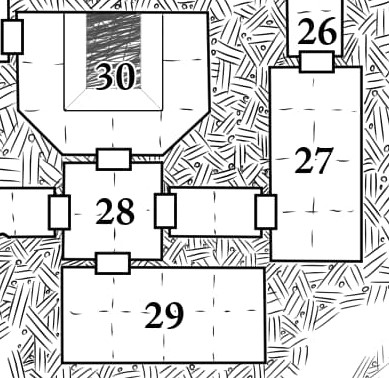
\includegraphics[width=\columnwidth]{pics/map_26-30.jpg}
\subsection{26 : Couloir}\label{n3:s26}
\begin{itemize}
  \item Couloir de 3m sur 6m, 3m de haut
  \item Mène à porte verrouillée :
  \begin{itemize}
    \item \textbf{Serrure aisée :} capacité voleur x2
    \item \textbf{Corrodée :} considérer comme une porte bloquée
  \end{itemize}
\end{itemize}

\subsection{27 : Salle des Esclaves}\label{n3:s27}
\begin{itemize}
  \item Salle de 6m sur 12m, haute de 3m
  \item Air \textbf{chaud et vicié}.
  \item Taches de sang et roche usée
  \item \textbf{Sifflement} constant au sud-est.
  \item \textbf{Entraves rouillées} au sol.
  \begin{itemize}
    \item Se referment aux jambes si à moins de 30cm
    \item Rouille : Brisées avec test de force
  \end{itemize}
\end{itemize}


\subsection{28 : Dôme}\label{n3:s28}
\begin{itemize}
  \item Salle de 6m sur 6m, haute de 6m
  \item Air \textbf{chaud et vicié}.
  \item \textbf{Sifflement} constant au nord.
  \item Plafond : \textbf{Dôme},  fresques d'hommes-serpents triomphants
  \item Porte au milieu de chaque mur.
  \item Porte sud verrouillée :
  \begin{itemize}
    \item Clef est au cou du Basilic (p. 14)
    \item Trop épaisse pour être brisée
  \end{itemize}
  \item Porte de pierre brisée à l'est.
  \item Porte de pierre entrouverte vers le nord.
\end{itemize}

\vfill

\subsection{29 : Salle du Trésor}\label{n3:s29}
\begin{itemize}
  \item Salle de 12m sur 6m, haute de 6m
  \item Contient tout ce que le MJ jugera bon de mettre au fond d'un donjon. [2000 PO au moins]
\end{itemize}

\subsection{30 : Fosse Sacrificielle}\label{n3:s30}
\begin{itemize}
  \item Salle de 12m sur 9m, haute de 6m
  \item Air vicié,
  \item \textbf{Flamme orangée} au nord, au fond d'une fosse profonde de 5m  aux parois en pente.
  \item Feu est alimenté par du gaz naturel acheminé depuis une antique mine perdue dans les tréfonds
  \item Chemin large de 60 cm borde le trou
  \item \textbf{Os carbonisés} couvrent le fond
  \item \textbf{Coulures d'or} sont visibles autour de la flamme
  \item \textbf{Pierres précieuses} couvertes de carbone (500 PO en tout) scintillent dans la lueur orangée du feu
  \item Si PJ entrent dans la fosse :
  \begin{itemize}
    \item -1D6 CON (temporaire, sauvegarde poison annule)
    \item 0 CON : inconscient, glisse jusqu'à la flamme :  2d6 dégâts de feu par round
  \end{itemize}
\end{itemize}

\vfill
\pagebreak


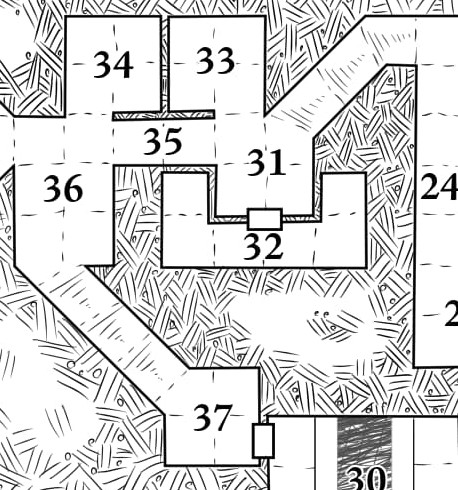
\includegraphics[width=\columnwidth]{pics/map_31-37.jpg}

\subsection{31 : Hall Gardé}\label{n3:s31}
\begin{itemize}
  \item Salle de 6m sur 6m, haute de 3m
  \item Sent la \textbf{poussière}
  \item Faible \textbf{cliquetis de chaîne} dans le lointain.
  \item Deux \textbf{statues de gardes} hommes-serpents aux coins sud
  \begin{itemize}
    \item Incroyablement \textbf{réalistes}
    \item Bien plus fines que tous les autres reliefs de la tombe
  \end{itemize}
\end{itemize}

Les statues sont des hommes-serpents pétrifiés, placés ici en guise de punition.
S'ils sont dé-pétrifiés, ils entrent dans une rage noire pendant 10 minutes, puis sombrent dans le désespoir.

Les statues peuvent se vendre 500 PO chacune dans une grande ville, ou 10 fois plus à un mage capable de reconnaître leur véritable nature.

\vfill

\subsection{32 : Salle d'Invocation}\label{n3:s32}
\begin{itemize}
  \item Salle de 12m sur 6m, haute de 3m, en forme de U
  \item Odeur de \textbf{vieux vin}, \textbf{papier brûlé} et \textbf{pourriture fongique}
  \item \'Enorme pile de débris bloque la porte.
  \begin{itemize}
    \item 30 minutes à déblayer,
    \item Très Bruyant
  \end{itemize}
  \item côté ouest, un \textbf{\nameref{monster:n3:succube}}
  \begin{itemize}
    \item \textbf{Non hostile}
    \item Prétend avoir été capturé par les gobelins et gardé prisonnier
    \item \textbf{Entravé} au pied (illusion)
    \item Au centre d'un cercle de confinement (difficile à voir)
    \begin{itemize}
      \item Brisé si franchi
    \end{itemize}
  \end{itemize}
  \item Petit \textbf{autel}
  \item 2 \textbf{bols en or} (150 PO chacun)
  \item \textbf{Dague magique} +1
  \item \textbf{Serpent de pierre} sinueux
  \begin{itemize}
    \item Magique
    \item Permet d'ouvrir la porte de \nameref{n3:s46}
  \end{itemize}
\end{itemize}

La pièce s'avère être une ancienne chambre d'invocation.
Baltoplate a été invoqué par les hommes-serpents pour répondre à leurs questions sur les enfers abyssaux.


\subsection{33 : Autel}\label{n3:s33}
\begin{itemize}
  \item Salle de 6m sur 6m, haute de 3m
  \item Sent légèrement l'\textbf{acide}.
  \item \textbf{Statue menaçante} à tête de cobra.
  \begin{itemize}
    \item Percée à sa base de deux trous assez larges pour laisser passer un bras humain
    \item \textbf{A du jeu :} peut pivoter.
    \item Sens anti-horaire : gaz empoisonné (1D6 dégâts, sauvegarde poison annule).
    \item Sens horaire : [2d1000 + 100 PO].
  \end{itemize}
\end{itemize}

\vfill
\pagebreak

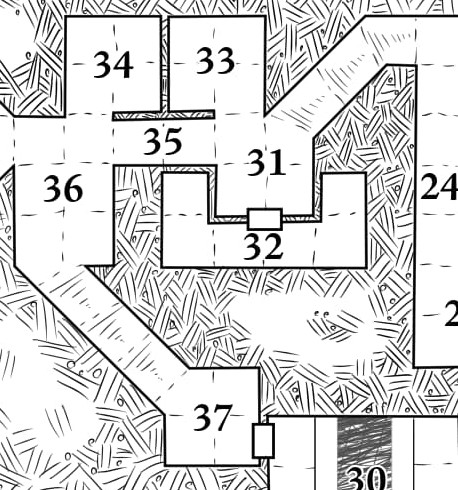
\includegraphics[width=\columnwidth]{pics/map_31-37.jpg}
\subsection{34 : Zone de Repos des Prêtres}\label{n3:s34}
\begin{itemize}
  \item Salle de 6m sur 6m, haute de 3m
  \item Odeur de \textbf{sang desséché}, de \textbf{tissus pourrissants} et de \textbf{champignons défraîchis}.
  \item Porte de bois a pourri sur place.
  \item 5 Coussins déchiquetés, maculés de sang
  \item \textbf{3 \oe ufs de pierre }
  \begin{itemize}
    \item Magiques
    \item Enduits de sang : chauffe (bouillotte) 8 heures
  \end{itemize}
\end{itemize}

\subsection{35 : Corridor Piégé}\label{n3:s35}
\begin{itemize}
  \item Couloir de 6m sur 3m, haut de 3m
  \item Sent la \textbf{poussière}.
  \item \textbf{4 sillons au plafond} évoquant le corps d'un serpent
  \item \textbf{Bandes de dalles} serpentent au sol.
  \begin{itemize}
    \item Marcher dessus : déclenche
    \item 4 pendules tranchants surgissent du plafond : 1D6 dégâts (sauvegarde mort annule)
    \item Pendant 3 round : si mouvement, doit esquiver un pendule
    \item Round 4 : tout s'écroule. 2D6 de dégâts (sauvegarde mort $\textonehalf$ dégâts)
  \end{itemize}
\end{itemize}

\vfill

\subsection{36 : Vestibule}\label{n3:s36}
\begin{itemize}
  \item Salle de 6m sur 9m, haute de 5m
  \item Sent le \textbf{tissu pourrissant}.
  \item Tintement de chaîne à l'ouest.
  \item Tentures partiellement pourries jonchent le sol
  \item Dallage à motifs géométriques.
  \item Se plaquer au mur ouest permet de se cacher du \textbf{\nameref{monster:n3:basilic}}.
  \item Couloir en pente vers le sud-est.
\end{itemize}


\subsection{37 : Fosse Piégée}\label{n3:s37}
\begin{itemize}
  \item Salle de 6m sur 6m, 3m de haut
  \item Air \textbf{froid}
  \item Carrelage de dalles :
  \begin{itemize}
    \item certaines cassées
    \item une manquante
  \end{itemize}
  \item \textbf{Piège :}
  \begin{itemize}
    \item Corniche large de 30 cm le long des murs \textbf{sûre}
    \item Autres carreaux ne sont soutenus que par de fines barres de métal
    \item Pied dans la zone centrale :
    \begin{enumerate}
      \item \textbf{Chute :} 1D6 dégâts (sauvegarde contre la mort annule)
      \item \textbf{Empalé} par les pics au fond : 1D6 dégâts (sauvegarde contre la mort annule)
    \end{enumerate}
  \end{itemize}
  \item Fosse vide
\end{itemize}

\vfill

\pagebreak

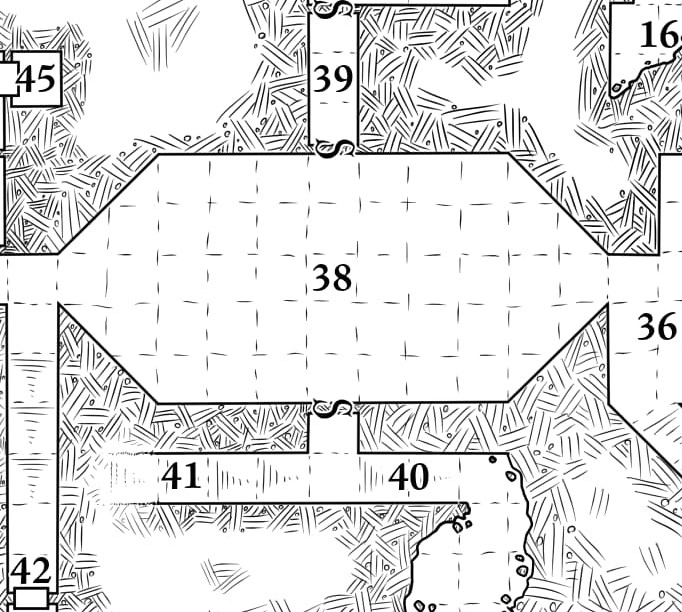
\includegraphics[width=\columnwidth]{pics/map_38-42.jpg}

\subsection{38 : Hall du Basilic}\label{n3:s38}
\begin{itemize}
  \item Grande salle de 34m sur 17m, haute de 15m
  \item Creusée à même la roche
  \item Air stagnant
  \item Tintements de chaîne
  \item Respiration à peine perceptible (\textbf{\nameref{monster:n3:basilic}})
  \item \textbf{8 piliers de roche}, certains détruits.
  \item \textbf{Statues de pierre} (araignées, gobelins, chauve-souris) détruites et parsemant le sol.
  \item Statues taillés avec une incroyable précision
  \item Mosaïques d'hommes-serpents triomphants sur les murs.
\end{itemize}

\subsection{39 : Passage Secret}\label{n3:s39}
\begin{itemize}
  \item Couloir de 3m sur 12m, 1.5m de haut
  \item Air stagnant, nuages de poussière.
  \item Taillé  à même la roche
  \item La porte devrait être invisible mais la mosaïque la cachant est endommagée et la \textbf{révèle}
  \item Mène en \textbf{\nameref{n2:s17}}
\end{itemize}


\subsection{40 : Passage Secret}\label{n3:s40}
\begin{itemize}
  \item Couloir de 3m sur 3m, 1.5m de haut
  \item Air aigre, relents immondes.
  \item \textbf{Intact}, caché par une mosaïque.
  \begin{itemize}
    \item \textbf{Difficile} à détecter
    \item Même principe que celle au nord : \textbf{localisable}
  \end{itemize}
  \item Murs lisses et soigneusement taillés
  \item Sol couvert de \textbf{ détritus gobelins}.
\end{itemize}

\subsection{41 : Escalier vers la Surface}\label{n3:s41}
\begin{itemize}
  \item Couloir de 10m sur 1m, 2.5m de haut
  \item Terreux, humide.
  \item Émerge entre les racines d'un arbre.
\end{itemize}

\subsection{42 : Porte en Cylindre}\label{n3:s42}
  \begin{itemize}
    \item Au bout d'un corridor de 3m sur 18m, 3m de haut
    \item Couloir en pente
    \item \textbf{Cylindre de roche} taillé d'une alcôve
    \begin{itemize}
      \item Peut accueillir deux personnes.
      \item Pivote dans les deux sens
      \item \textbf{Sens anti-horaire :} l'alcôve arrive face à des lances jaillissant de la roche
      pour transpercer les occupants (1d6 dégâts par round).
      \item \textbf{Sens horaire :} autel avec idole de pierre portant 2 bols en or (100 PO chaque).
      \item \textbf{180 degrés :} débouche sur \nameref{n3:s47}
    \end{itemize}
\end{itemize}

\vfill\pagebreak
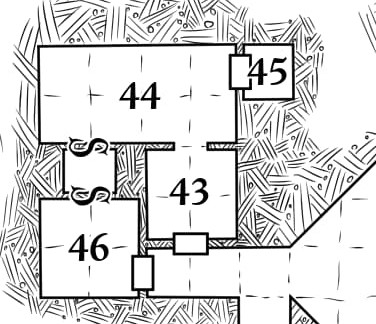
\includegraphics[width=\columnwidth]{pics/map_43-46.jpg}

\subsection{43 : Antichambre de Xiximantre}\label{n3:s43}
\begin{itemize}
  \item Salle de 6m sur 6m, 5m de haut
  \item Relents âcres, milles odeurs
  \item Taillée à même la roche
  \item Bas-reliefs de pierre noire.
  \item Lampes magiques violacées incrustées dans les murs
  \item Présence de  \textbf{\nameref{monster:n3:xiximanter}}
\end{itemize}

\subsection{44 : Réserve à Ingrédients}\label{n3:s44}
\begin{itemize}
  \item Salle de 12m sur 6m, 5m de haut
  \item Relents âcres, milles odeurs
  \item Lampes magiques violacées incrustées dans les murs
  \item Barils, caisses, cercueils, flacons, bottes d'herbes.
  \begin{itemize}
    \item Une fiole contient du safran en poudre (2000 PO)
    \item Une petite bouteille renferme  1d10 graines d'une espèce de plante à présent disparue (300 PO chacune)
  \end{itemize}
  \item Six oubliettes à couvercles de bronze sont incrustées dans le sol
  \item Une contient  1d10 Gobelins Fongiques.
  \item Passage secret derrière les caisses
\end{itemize}

Xiximantre ne cédera rien de son stock à moins d'obtenir en échange des ingrédients d'encore plus grande rareté ou valeur

\vfill

\subsection{45 : Laboratoire à Potions}\label{n3:s45}
\begin{itemize}
  \item Salle de 3m sur 3m, 3m de haut
  \item Lampes magiques violacées, bouillonnement,
  \item Éprouvettes alchimiques, verrerie poussiéreuse et étagères luisantes de magnifiques flacons.
  \item Porte de fer verrouillable.
  \item À peine assez de place pour travailler.
  \item Sur les étagères :
  \begin{itemize}
    \item 2 potions de mutation de sort
    \item 1 potion d'immortalité modérée (1d100 + 20 années de vie naturelle supplémentaires)
    \item 1 potion de poison indétectable (aucun goût mais tue (pas de jet de sauvegarde) en 1 minute)
    \item 2 potions de soin
    \item 1d10 + 10 potions aléatoires
  \end{itemize}
\end{itemize}

Xiximantre n'autorisera pas les PJ à y accéder à moins qu'ils n'acceptent de devenir ses apprentis (ou victimes)

Ses potions les plus puissantes prennent des décennies à élaborer.
Il est prêt à échanger ses concoctions contre des créatures vivantes, sorts, ingrédients rares et apprentis.
Il n'acceptera ni monnaie ni trésors.

Si les aventuriers transportent ouvertement des objets pillés dans la tombe, cela éveillera ses soupçons et il tentera de les empoisonner, capturer ou manipuler.

\subsection{46 : Salle du Trône}\label{n3:s46}
\begin{itemize}
  \item Salle de 6m sur 6m, 6m de haut
  \item Sent la poussière et les copeaux de métal.
  \item La porte est faite de \textbf{serpents de pierre} entremêlés.
  \begin{itemize}
    \item L'un est manquant, en \textbf{\nameref{n3:s32}}.
    \item Si remis en place, la porte glisse et s'ouvre silencieusement
  \end{itemize}
  \item Murs de roche rouge, ornée d'ors et de \textbf{miroirs}
  \item Murs décorés d'écailles joliment gravées.
  \begin{itemize}
    \item 8 miroirs de la taille d'une main dressés sur des présentoirs en bois : 100 PO chaque
    \item trône : 2500 PO.  3 personnes pour le soulever
  \end{itemize}
  \item \textbf{Passage secret} derrière une tenture pourrissante.
\end{itemize}

Si les PJ utilisent le passage secret, le sorcier sera surpris, ainsi que furieux s'ils ne parviennent pas à donner une excuse plausible.

\vfill\pagebreak
\ifmulticolEnd
\begin{center}
  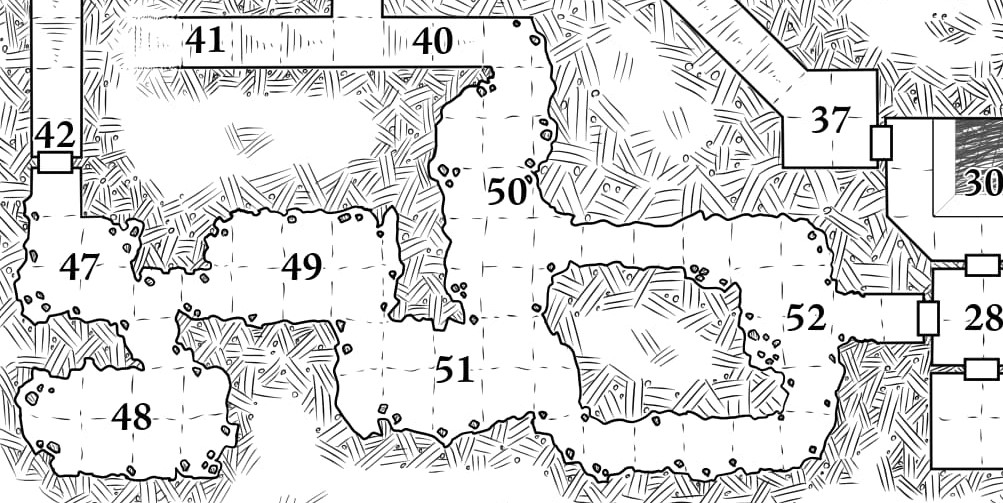
\includegraphics[width=\linewidth]{pics/map_47-52.jpg}
\end{center}
\ifmulticolStart

\subsection{47 : Terrier Gobelin}\label{n3:s47}
\begin{itemize}
  \item Salle de 6m sur 6m, 1.5m de haut
  \item Empeste le graillon, les champignons, la pourriture et l'humidité.
  \item Chuchotis.
  \item Sol couvert de scarabées
  \item Des détritus jusqu'au mollet.
  \item Fouille des débris :
  \begin{itemize}
    \item 2d6 couteaux d'argent (10 PA chaque)
    \item PJ couvert de fange et guano
  \end{itemize}
  \item Stock de plumes, chiffons et bols de graisse
\end{itemize}

\subsection{48 : Fosse de Génération de Gobelins}\label{n3:s48}
\begin{itemize}
  \item Salle de 12m sur 6m, 1.5m de haut
  \item Pestilence fongique, animaux pourrissants, gobelins à demi formés.
  \item \textbf{Spectacle répugnant :} Jet de sauvegarde contre le poison ou fuite avec nausée
\end{itemize}

La fosse réincarne les âmes des gobelins fongiques morts, c'est l'une des expériences ratées de
\textbf{\nameref{monster:n3:xiximanter}}, censée apporter l'immortalité.

Aucun trésor ici, mais tant que cette salle n'est pas incendiée, le nombre de gobelins dans le donjon sera toujours \emph{"beaucoup trop de gobelins"}.

\vfill

\subsection{49 : Salle du Trône Gobeline}\label{n3:s49}
\begin{itemize}
  \item Salle de 9m sur 6m, 1.5m de haut
  \item Chuchotis, bruits de scarabées écrasés
  \item 1d6 (explosif) \textbf{\nameref{monster:n3:gob}} présents
  \begin{itemize}
    \item Mangent des chauves-souris, se battent ou vénèrent leur roi actuel
    \item Si aucun Roi : vénèrent une idole sculptée en boue et brindilles
  \end{itemize}
  \item \textbf{Couronne gobeline :} faite de bâtons et couverts tordus
\end{itemize}


\subsection{51 : Dortoir Gobelin}\label{n3:s51}
\begin{itemize}
  \item Salle de 15m sur 6m, 1.5m de haut
  \item Crasse, pourriture, chuchotis
  \item Statues grossières de boue et bâtons.
  \item \textbf{Nuit :} 1d6 (explosif) \textbf{\nameref{monster:n3:gob}}
  \item \textbf{Jour :} 3d6+10 (explosif) \textbf{\nameref{monster:n3:gob}}
  \begin{itemize}
    \item Presque \textbf{invisibles} parmi les débris.
    \item \textbf{Endormis}
    \item \textbf{Bruit :} se réveillent en 2 rounds
  \end{itemize}
\end{itemize}

\vfill
\pagebreak

\ifmulticolEnd
\begin{center}
  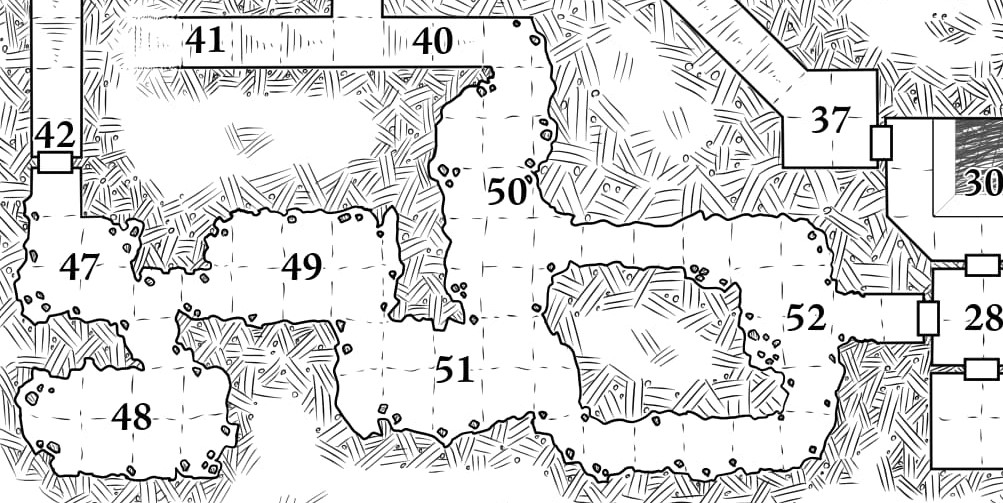
\includegraphics[width=\linewidth]{pics/map_47-52.jpg}
\end{center}
\ifmulticolStart

\subsection{50 : Fermes Gobelines}\label{n3:s50}
\begin{itemize}
  \item Salle de 6m sur 12m, 1.5m de haut
  \item Plantes en putréfaction, puanteur du fumier, spores de champignons
  \item Sol inégal
  \item Des détritus jusqu'aux genoux
  \item Les \textbf{\nameref{monster:n3:gob}} plantent tout et n'importe quoi
  \item \textbf{Fouille} (1 tour par carré de 1.5m) :
  \begin{enumerate}
    \item Un doigt et une fourchette
    \item Une dague rouillée
    \item 2D100 PO
    \item Rubis (300 PO)
    \item Des os de poulet
    \item \textbf{Couronne des rois serpents}
  \end{enumerate}
\end{itemize}

Les apothicaires et sorciers expérimentés peuvent identifier les champignons bleus poussant ici comme des concombres des donjons, capables de guérir la pétrification en 1d6 jours une fois coupés en rondelles et frottés contre la peau.

\vfill
\
\begin{highlight}[Couronne des rois serpents]
  \begin{itemize}
    \item Composée de 8 petits serpents d'or et platine entremêlés, aux yeux d'émeraude et dents de diamant
    \item 3000 PO de matériaux
    \item \textbf{Magique :}
    \begin{itemize}
      \item \textbf{Si portée :} sauvegarde contre les sorts, ou être prostré et terrifié une heure
      \item \textbf{3 échecs} consécutifs : état permanent
    \end{itemize}
  \end{itemize}
\end{highlight}

\subsection{52 : Salle de Garde des Gobelins}\label{n3:s52}
\begin{itemize}
  \item Salle de 6m sur 6m, 1.5m de haut
  \item Air vicié
  \item Pourriture en train de sécher
  \item Stock d'armes \textbf{\nameref{monster:n3:gob}}
  \begin{itemize}
    \item 2 fourches,
    \item Une pile de couverts en argent (200 PO)
    \item des douzaines de bâtons affûtés
  \end{itemize}
  \item 1 \textbf{\nameref{monster:n3:gob}} fait le guet
  \begin{itemize}
    \item Armé d'un balai
    \item \'Eloigne les \textbf{\nameref{monster:n3:squelgel}}
    \item Repousse les PJ si arrivent du \textbf{\nameref{n3:s28}}
    \item S'enfuit en hurlant si les PJ arrivent du \textbf{\nameref{n3:s28}}
  \end{itemize}
\end{itemize}
